\section{绪论}

\subsection{背景与意义}

\textbf{金融市场波动率}（以下简称波动率）是衡量资产价格不确定性和市场风险状态的重要指标，在风险管理、资产配置、衍生品定价以及金融监管中具有重要作用。Andersen et al. (2003)指出，与收益率水平相比，金融资产收益率的波动率通常表现出更强的可预测性。大量金融计量研究表明，资产收益率序列普遍存在尖峰厚尾、波动聚集和条件异方差等特征，即高波动时期往往更可能伴随较高的未来波动，而低波动时期则更可能延续低波动状态。除条件异方差外，金融波动率还具有明显的多尺度持续性。不同类型投资者具有不同投资期限和信息处理周期，短期交易者、中期投资者和长期机构投资者共同作用，使市场波动率同时受到日度、周度和月度历史波动状态影响。基于这些原因，对于波动率的预测研究在近年来已成为金融学科中的一个重要研究方向。

宏观政策环境可能通过投资者预期、风险偏好和流动性与市场波动相关。EPU 是新闻文本中的政策不确定性测度，不能直接等同于外生政策冲击。本文检验含 EPU 的残差修正组合是否与预测表现改善相伴，而不预设因果传导机制。

基于上述背景，本文以沪深 300 成份指数（CSI 300 Index）为主要研究对象，构建了 XGB-MIDAS-EPU-DEC 模型。该模型检验政策不确定性与波动率代理预测误差之间的潜在关联，为股指波动率的点预测与区间预测提供了一种潜在的研究框架。

\subsection{研究现状}

围绕金融市场波动率预测，既有研究大致可以分为 4 类：传统条件异方差模型、实现波动率与 HAR 类模型、经济政策不确定性与金融市场波动研究，以及机器学习金融预测与预测评价研究。

第一类研究是基于条件异方差结构的传统计量模型。金融资产收益率通常具有尖峰厚尾、波动聚集和条件异方差等特征，早期线性时间序列模型难以刻画收益率方差随时间变化的特征，因此条件异方差模型成为金融波动率建模的重要基础。Engle 提出的 ARCH 模型首次将条件方差设定为历史扰动平方项的函数，为刻画时间变动波动率提供了系统方法 \citep{Engle1982}。Bollerslev 在此基础上提出 GARCH 模型，使条件方差同时依赖滞后扰动平方项和滞后条件方差项，从而以较为简洁的结构刻画波动率持续性 \citep{Bollerslev1986}。由于 GARCH(1,1) 模型结构简洁、解释清晰且在实证中具有较强竞争力，本文将其作为传统基准模型之一。

第二类研究关注实现波动率和多尺度波动结构。随着高频金融数据的使用，Andersen、Bollerslev、Diebold 和 Labys 将高频日内收益率与日度及更低频率波动率测度联系起来，推动了已实现波动率（Realized Volatility）在波动率预测中的应用 \citep{AndersenBollerslevDieboldLabys2003}。在此基础上，Corsi 提出的 HAR-RV 模型通过日度、周度和月度三个波动率成分刻画金融市场中的异质投资者结构和多尺度波动持续性 \citep{Corsi2009}。虽然本文未使用高频数据构造标准已实现波动率，但仍借鉴 HAR 模型的多尺度思想，使用日度平方收益率代理变量构造类 HAR 基准模型，以刻画短期、周度和月度波动信息对未来波动率的影响。

第三类研究关注经济政策不确定性与金融市场波动之间的关系。Baker、Bloom 和 Davis 基于报纸文本构造 EPU 指数，发现政策不确定性与股票市场波动、企业投资和宏观经济活动存在密切联系 \citep{BakerBloomDavis2016}。Liu 和 Zhang 进一步研究了 EPU 对股票市场波动率的预测作用，发现将 EPU 纳入波动率预测模型能够改善样本外预测能力 \citep{LiuZhang2015}。针对中国市场，Davis、Liu 和 Sheng 基于《人民日报》和《光明日报》两份中国大陆报纸构造了中国 EPU 指标，使研究中国政策不确定性与金融市场关系具有了更贴近本土语境的数据基础 \citep{DavisLiuSheng2019}。这类研究说明，政策不确定性不仅是宏观经济研究中的背景变量，也可能是金融市场风险预测中的有效信息来源。

第四类研究关注机器学习方法、预测评价和区间预测。机器学习模型能够较灵活地刻画变量之间的非线性关系和交互效应。Gu、Kelly 和 Xiu 在资产定价研究中系统比较了多种机器学习方法，表明机器学习模型在处理高维预测变量和非线性关系方面具有优势 \citep{GuKellyXiu2020}。Chen 和 Guestrin 提出的 XGBoost 通过正则化目标函数、树结构约束、学习率控制、列采样和行采样等机制，在提升预测能力的同时控制过拟合风险 \citep{ChenGuestrin2016}。但是，金融时间序列噪声较强、样本有限且结构变化频繁，机器学习模型必须通过严格的样本外预测设计进行验证。

预测评价是衡量模型好坏的重要根据，波动率预测研究不能仅依赖单一误差指标。MSE 更强调较大误差，MAE 对极端误差相对稳健，而 QLIKE 常用于方差预测评价。Patton 指出，当真实波动率不可观测、只能使用代理变量时，损失函数选择会影响预测比较结论，在代理变量条件无偏等适用前提下，QLIKE可提供对代理噪声较稳健的模型排序；本文将其作为方差尺度评价指标 \citep{Patton2011}。此外，Diebold 和 Mariano 提出的预测精度比较检验为非嵌套模型的样本外预测比较提供了经典方法 \citep{DieboldMariano1995}；Clark 和 West 针对嵌套预测模型提出修正检验方法，适用于比较扩展模型是否在样本外显著优于基准模型 \citep{ClarkWest2007}。

近年来，区间预测也逐渐成为金融预测研究中的重要内容。Christoffersen 提出了评价区间预测的经典框架，强调覆盖率和独立性是区间预测有效性的重要维度 \citep{Christoffersen1998}。Gneiting 和 Raftery 从严格适当评分规则角度讨论预测分布评价，为综合考察校准性与尖锐性提供了理论基础 \citep{GneitingRaftery2007}。共形预测为模型无关的预测区间构造提供了新的方法。Vovk、Gammerman 和 Shafer 系统阐述了共形预测的理论基础 \citep{Vovk2005}，Shafer 和 Vovk 对共形预测方法进行了教程式介绍 \citep{ShaferVovk2008}，Lei et al. 进一步发展了回归问题中的分布无关预测推断框架 \citep{Lei2018}。不过，标准共形预测通常依赖可交换性假设，而金融时间序列存在自相关、波动聚集和分布漂移，严格意义上并不满足该条件。Xu 和 Xie 针对动态时间序列提出共形预测区间方法，为依赖数据中的序贯预测区间构造提供了重要参考 \citep{XuXie2021}。因此，本文在区间预测部分采用滚动校准思想，重点从经验覆盖率、区间宽度和区间得分等角度评价模型表现，而不将其解释为严格满足标准共形预测理论条件下的无条件有效区间。

现有文献提供了点预测、区间预测与混频建模的方法基础。本文在历史追溯与修订重分析中联合考察这些维度；未进行系统综述来证明此类研究稀缺，也不主张提出普遍最优的预测模型。

\subsection{主要研究内容}

围绕中国股指波动率预测任务，基于上述研究现状，本文的研究内容主要包括以下 3 个方面：

第一，整理日度行情与月度 EPU，构建 XGB-Market 及含历史残差、MIDAS-EPU 的误差修正组合，并与类 HAR 和 GARCH(1,1) 比较。修订版增加只含历史残差的XGB-AR消融对照，检验加入EPU后的指标变化；不把相关预测改善解释为因果效应。

第二，以MSE、MAE和QLIKE评价点预测，对18项损失差报告HAC及Holm调整诊断，明确其回顾性和近似嵌套推断限制。对五模型采用相同的滚动残差区间构造，评价覆盖率、宽度与区间得分；该结果不等同于 GARCH 原生分布预测区间的比较。

第三，用上证50与纳斯达克综合指数进行替代样本检查。金融预测存在数据窥探与多重比较风险\citep{HarveyLiuZhu2016,LoMacKinlay1990}；少量替代样本只能提供初步外部证据，不能排除数据选择偏差或证明普适性。

本文的整体流程如图 \ref{fig:f}所示：

\begin{figure}[htbp]
	\centering
	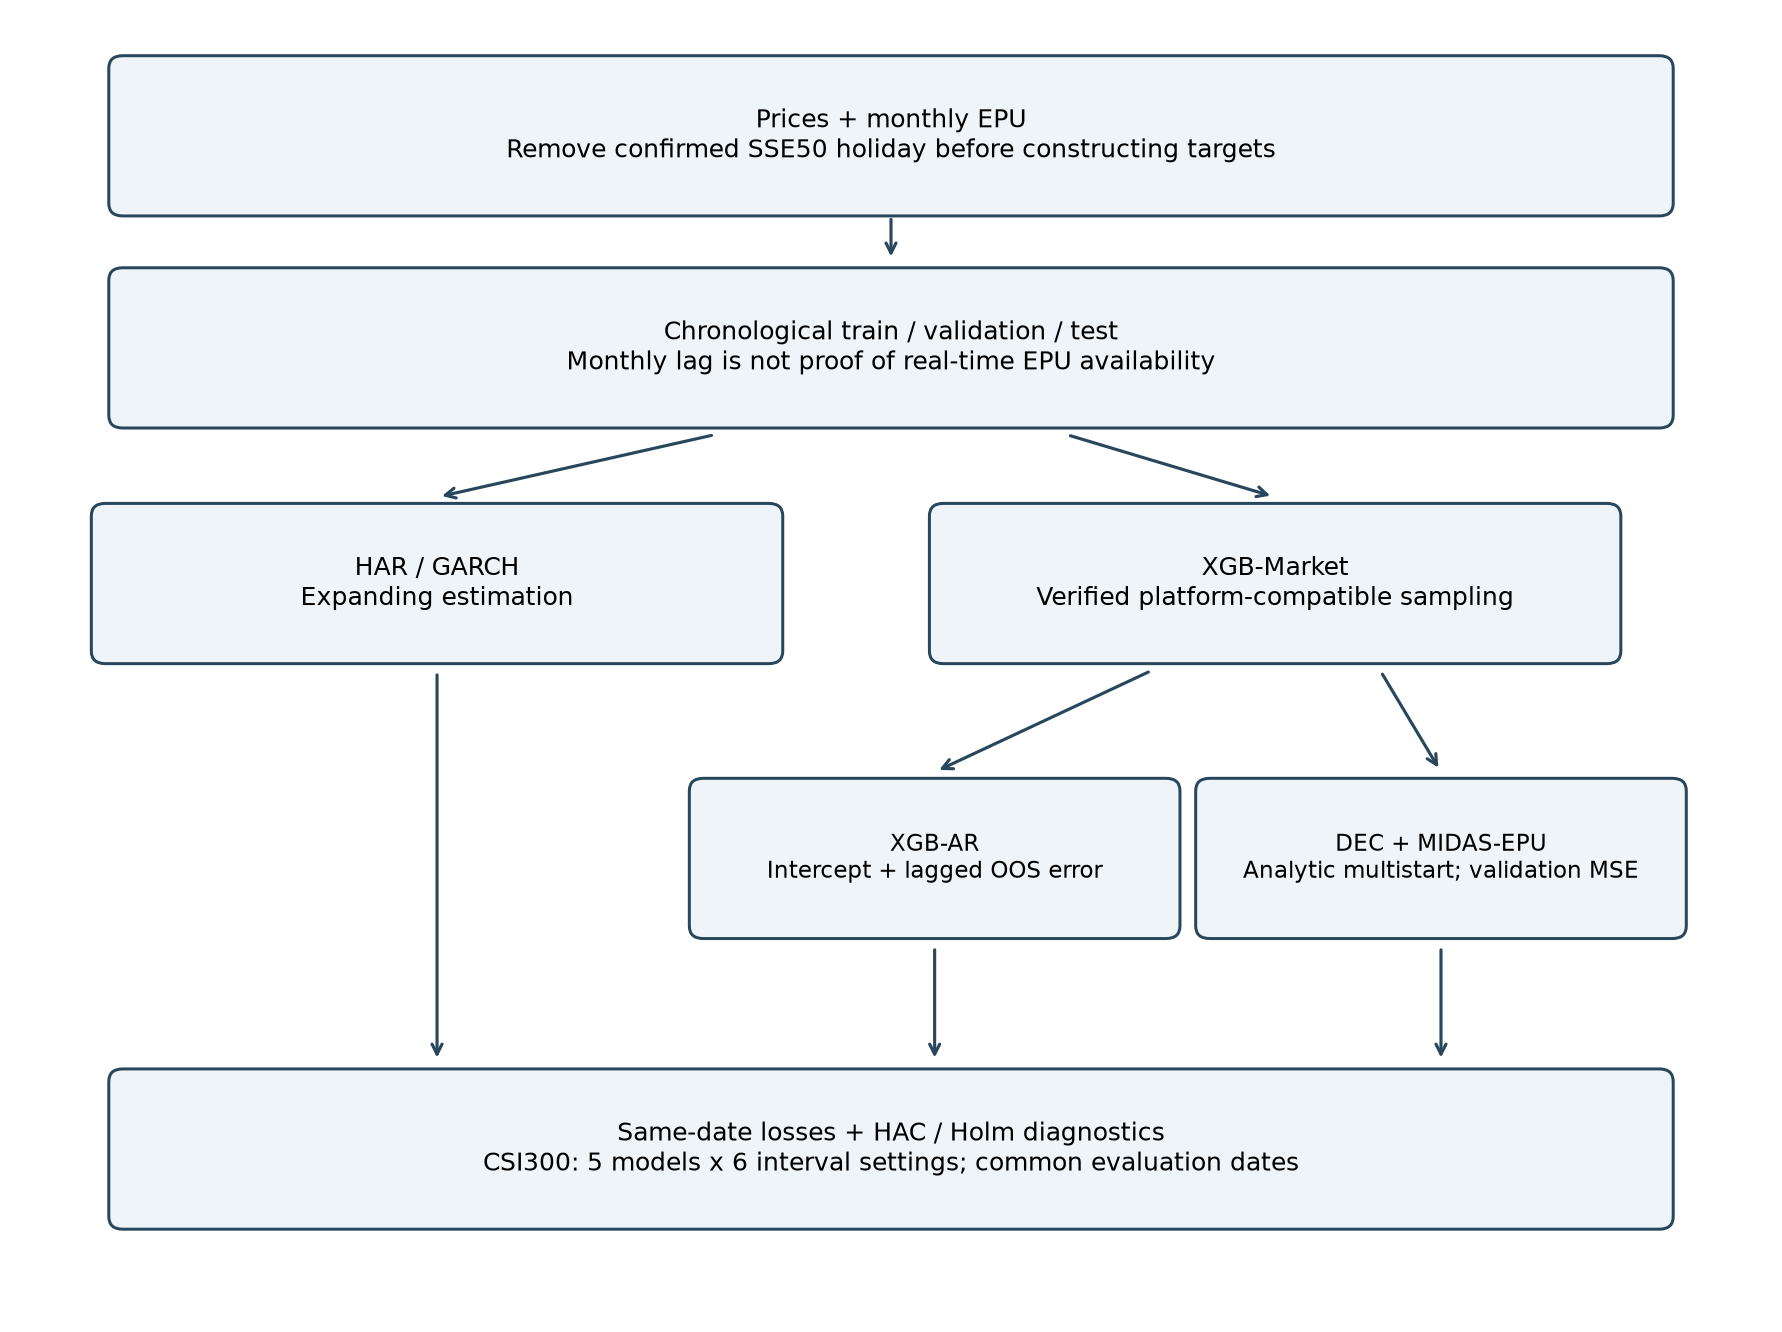
\includegraphics[width=1\textwidth]{../../results/revised/method_flow.png}
	\caption{修订研究流程：稳定求解、消融比较与共同日期评价}
	\label{fig:f}
\end{figure}


	
		
		
		
		
		
		
		
		
		
		
		
		
		
		
		
	


\subsection{本文组织结构}

本文共分为 5 章，具体安排如下：

第一章为绪论，主要介绍研究背景与意义、研究现状、研究内容与技术路线以及全文结构安排。

第二章为带动态误差修正机制的股指波动率预测模型，提出并详细推导了 XGB-MIDAS-EPU-DEC 混合预测模型，同时系统梳理了用于对比分析的各类基准模型。在此基础上，本章详细说明本文实证研究的数据来源与实验设计方案，并系统定义了点预测与区间预测的多维度评价指标体系，为后续的实证检验与结果分析奠定方法基础。

第三章为波动率点预测精度分析与结果检验，比较 XGB-MIDAS-EPU-DEC 模型和各类基准模型在 CSI 300 指数样本中的点预测表现，分析预测路径、损失函数结果、统计检验结果和 MIDAS-EPU 权重机制。

第四章为波动率区间预测精度分析与结果检验，基于滚动共形预测方法构造波动率预测区间，并从经验覆盖率、平均区间宽度、区间得分和覆盖检验等角度评价不同模型的区间预测表现。

第五章为 XGB-MIDAS-EPU-DEC 模型在其他样本下的稳健性分析，以上证 50 指数和纳斯达克综合指数作为替代样本，在相同实验框架下重复主要模型比较，以检验本文结论是否具有跨指数稳健性。